\chapter{Dependent Types --- When Types Depend on Values}
\label{ch:dependent-types}

\begin{keyinsight}[Chapter Milestone]
This is one of the most important chapters in the book. Dependent types represent the apex of type system expressiveness: types that \emph{depend on values}. Everything we have built so far --- simple types, polymorphism, type classes, type constructors --- has been leading here. By the end of this chapter you will understand why languages like Agda, Idris, Coq, and Lean are so powerful, and you will recognize dependent typing hiding inside ordinary \cpp{} features you already use.
\end{keyinsight}

\section{What We Can Express So Far --- And What We Cannot}

Let us take stock. In the previous chapters we covered a great deal of ground. We have simple types: \typename{Int}, \typename{Bool}, \typename{String}. We have function types: $A \to B$. We have product types and sum types. We have polymorphism --- type variables, letting us write a single \typename{identity} function that works for every type. We can write \typename{List}$\langle A \rangle$ and \typename{Maybe}$\langle A \rangle$ and \typename{Pair}$\langle A, B \rangle$, where the type \emph{depends on another type}.

All of that is genuinely powerful. But there is a wall we keep running into.

Consider a simple programming problem: write a function that takes a list and returns the first element. In Haskell:

\begin{lstlisting}[style=haskell]
head :: [a] -> a
head (x:_) = x
head []    = error "head: empty list"  -- BOOM
\end{lstlisting}

That \code{error} call is a runtime crash waiting to happen. The type signature \code{[a] -> a} makes a promise the type system cannot enforce: it says ``give me a list and I will give you an element,'' but it silently fails when the list is empty. The type system has no way to say ``give me a \emph{non-empty} list.''

Or consider vectors and matrices. Suppose you want to write a dot product function:

\begin{lstlisting}[style=cpp]
double dot_product(std::vector<double> a, std::vector<double> b) {
    // What if a.size() != b.size()? Runtime error? Undefined behavior?
    double result = 0.0;
    for (size_t i = 0; i < a.size(); i++)
        result += a[i] * b[i];  // b[i] might be out of bounds!
    return result;
}
\end{lstlisting}

The type \code{std::vector<double>} says nothing about the \emph{length} of the vector. We cannot express at the type level that both vectors must have the same length. We either write a runtime check (and throw an exception), silently read garbage memory, or add a comment that says ``caller must ensure lengths match'' --- and hope.

Matrix multiplication is even more painful. Multiplying an $m \times k$ matrix by a $k \times n$ matrix gives an $m \times n$ matrix. The inner dimensions must match. This constraint is mathematically precise and checkable at compile time --- but not in any type system we have seen so far. The type \code{Matrix} or even \code{Matrix<double>} cannot encode the dimensions.

\begin{intuition}
The pattern is always the same. We want to write down a type that \emph{says something about a specific value} --- a specific length, a specific size, a specific index bound. Simple polymorphism lets types depend on \emph{other types} (like \code{List<A>} where \code{A} is a type). But we want types to depend on \emph{values}, like lengths and indices.
\end{intuition}

This is the gap that dependent types fill. A dependent type is a type that is indexed by, or computed from, an ordinary value at the term level. And this single idea --- apparently simple, almost obvious once you see the need --- opens up a universe of expressive power.

\section{The Key Idea: Types That Contain Values}

Let us think about what we want. We want a type \typename{Vec}$(A, n)$ that means ``a vector of exactly $n$ elements of type $A$.'' Here $A$ is a type (as before), but $n$ is a \emph{natural number value}. The type depends on $n$.

\begin{definition}[Dependent Type]
A \textbf{dependent type} is a type that is parametrised by a value. If $A$ is a type and $B$ is a function from values of type $A$ to types, then $B$ is called a \textbf{type family} over $A$. We write $B(x)$ for the type that $B$ assigns to the value $x : A$.
\end{definition}

Some examples to make this concrete:

\begin{itemize}
    \item $\text{Vec}(A, n)$ --- the type of vectors of length exactly $n$, with elements of type $A$. Here $n : \Nat$ (a natural number value) is part of the type.
    \item $\text{Matrix}(A, m, n)$ --- the type of $m \times n$ matrices with entries of type $A$. The dimensions $m, n : \Nat$ are in the type.
    \item $\text{Fin}(n)$ --- the type of natural numbers strictly less than $n$. This is the canonical type of safe array indices. $\text{Fin}(5)$ has exactly five inhabitants: $0, 1, 2, 3, 4$.
    \item $\text{Proof}(P)$ --- the type of proofs of the proposition $P$. A value of this type is evidence that $P$ is true. (We will come back to this remarkable idea.)
\end{itemize}

Now consider what we can do with \typename{Vec}. We can give \code{head} a type that is actually safe:

\[
\text{head} : \Pi(n : \Nat).\; \text{Vec}(A, n+1) \to A
\]

Read this as: ``for any natural number $n$, a function that takes a vector of length $n+1$ and returns an element of type $A$.'' The type \emph{requires} the vector to have at least one element ($n+1$ is always at least 1). You simply cannot call this function on an empty vector --- the \emph{types} will not let you. The crash is impossible by construction.

Or for dot product:

\[
\text{dotProduct} : \Pi(n : \Nat).\; \text{Vec}(\mathbb{R}, n) \to \text{Vec}(\mathbb{R}, n) \to \mathbb{R}
\]

Both arguments must have the \emph{same} length $n$. Passing vectors of different lengths is a \emph{type error}, caught at compile time, not a runtime crash.

\begin{keyinsight}[Precision Through Values in Types]
Dependent types let the type system be as precise as your mathematical specification. Every constraint you can state mathematically about values --- ``these two lengths must match,'' ``this index must be in bounds,'' ``this list must be non-empty'' --- can potentially be enforced at the type level, turning runtime errors into compile-time errors.
\end{keyinsight}

\section{Dependent Function Types: Pi Types}

The central construction in dependent type theory is the \textbf{dependent function type}, also called a \textbf{Pi type} (written $\Pi$).

\begin{definition}[Pi Type / Dependent Function Type]
Given a type $A$ and a type family $B$ indexed by $A$ (i.e., for each $x : A$, there is a type $B(x)$), the \textbf{Pi type} is:
\[
\Pi(x : A).\; B(x)
\]
A function of this type takes a value $x : A$ and returns a value of type $B(x)$. Crucially, the \emph{return type depends on the input value}.
\end{definition}

The notation varies across systems. You will also see:
\begin{itemize}
    \item $(x : A) \to B(x)$ \quad (Agda, Idris notation)
    \item \code{forall (x : A), B x} \quad (Coq/Rocq, Lean notation)
    \item $\prod_{x : A} B(x)$ \quad (mathematical notation)
\end{itemize}

The Pi type is a \emph{generalisation} of the ordinary function type. If $B(x)$ does not actually depend on $x$ --- that is, $B(x) = B$ for all $x$ --- then $\Pi(x : A).\, B(x)$ is just $A \to B$, an ordinary function type.

But here is something even more striking: the Pi type also generalises \emph{polymorphism}. In System F (Chapter 7), we wrote $\forall \alpha.\, T(\alpha)$ for ``for all types $\alpha$, a value of type $T(\alpha)$.'' This is exactly a Pi type where the domain is the universe of types! In dependent type theory, types are values too, and we can quantify over them with the same $\Pi$ that we use for ordinary values.

\begin{intuition}
$\Pi(x : A).\, B(x)$ unifies three things you already know:
\begin{itemize}
    \item \textbf{Ordinary functions} $A \to B$: when $B$ does not depend on $x$.
    \item \textbf{Polymorphic functions} $\forall \alpha.\, T(\alpha)$: when $A$ is a universe of types.
    \item \textbf{Dependent functions}: the new case, when $B$ genuinely depends on the value $x$.
\end{itemize}
\end{intuition}

Let us look at some concrete Pi-typed functions.

\subsection*{Example: replicate}

The function \code{replicate} takes a number $n$ and a value $a : A$, and produces a vector of $n$ copies of $a$:
\[
\text{replicate} : \Pi(n : \Nat).\; \Pi(A : \Type).\; A \to \text{Vec}(A, n)
\]
In Idris syntax:
\begin{lstlisting}[style=haskell]
-- Idris 2
replicate : (n : Nat) -> a -> Vect n a
replicate 0     _ = []
replicate (S n) x = x :: replicate n x
\end{lstlisting}

When you call \code{replicate 5 'a'}, the return type is \code{Vect 5 Char} --- a vector of exactly 5 characters. The $5$ is part of the type!

\subsection*{Example: append}

Appending two vectors. If you append a vector of length $m$ to a vector of length $n$, you get a vector of length $m + n$. The return type is computed from the input values:

\begin{lstlisting}[style=haskell]
-- Idris 2
append : Vect m a -> Vect n a -> Vect (m + n) a
append []      ys = ys
append (x::xs) ys = x :: append xs ys
\end{lstlisting}

The type \code{Vect (m + n) a} contains an \emph{arithmetic expression} involving the input values $m$ and $n$. The type checker must verify that the implementation is consistent with this claim --- it must reason about arithmetic. This is why dependent type checkers include substantial machinery for normalising and comparing expressions.

\subsection*{Example: safe vector lookup}

\begin{lstlisting}[style=haskell]
-- Idris 2
-- Fin n is the type of numbers < n (safe indices into Vect n)
index : Fin n -> Vect n a -> a
index FZ     (x :: _)  = x
index (FS i) (_ :: xs) = index i xs
\end{lstlisting}

\code{Fin n} is the type of natural numbers strictly less than $n$. It has exactly $n$ inhabitants. You \emph{cannot} construct a value of type \code{Fin 0} (there are no numbers less than 0), so \code{index} on an empty vector is literally impossible to call --- the type of the index argument prevents it.

\section{Dependent Pair Types: Sigma Types}

The companion to the Pi type is the \textbf{dependent pair type}, also called the \textbf{Sigma type} (written $\Sigma$).

\begin{definition}[Sigma Type / Dependent Pair Type]
Given a type $A$ and a type family $B$ over $A$, the \textbf{Sigma type} is:
\[
\Sigma(x : A).\; B(x)
\]
A value of this type is a \textbf{pair} $(a, b)$ where $a : A$ and $b : B(a)$. The type of the second component depends on the \emph{value} of the first component.
\end{definition}

Again, this generalises familiar things:
\begin{itemize}
    \item \textbf{Ordinary pairs} $A \times B$: when $B(x) = B$ for all $x$ (the second type does not depend on the first value).
    \item \textbf{Existential types} $\exists \alpha.\, T(\alpha)$: when $A$ is the universe of types (``there exists some type $\alpha$ together with a value of type $T(\alpha)$'').
    \item \textbf{Dependent pairs}: the new case, when the second type genuinely depends on the first value.
\end{itemize}

\begin{intuition}
A Sigma type $\Sigma(x : A).\, B(x)$ packages a value together with \emph{evidence} or \emph{data} that depends on that value. The first component is a witness; the second component is related data whose type is determined by the witness.
\end{intuition}

\subsection*{Example: Dynamically-sized vector}

Consider $\Sigma(n : \Nat).\, \text{Vec}(A, n)$. A value of this type is a pair: a natural number $n$ together with a vector of \emph{exactly} that length. This is essentially what \code{std::vector<A>} is at runtime --- a length plus a buffer of that length --- except that in the dependent type version, the relationship between the two components is enforced by the type system.

This is a remarkably clean way to think about dynamic arrays: they are elements of $\Sigma(n : \Nat).\, \text{Vec}(A, n)$, with the length as a first-class part of the value.

\subsection*{Example: Bounded natural numbers}

$\Sigma(n : \Nat).\, n < 100$ is the type of natural numbers that are less than 100. A value is a pair: a number $n$ together with a proof that $n < 100$. This is not just documentation --- it is a machine-checked proof embedded in the value.

\subsection*{Example: Non-empty lists}

We can define non-empty lists as $\Sigma(\text{xs} : \text{List}(A)).\, \text{xs} \neq []$: a list together with a proof that it is non-empty. Then \code{head} on this type is total and safe:
\[
\text{head} : \Sigma(\text{xs} : \text{List}(A)).\, \text{xs} \neq [] \to A
\]

\begin{keyinsight}[Sigma Types as Specifications]
A Sigma type $\Sigma(x : A).\, P(x)$ captures the idea of a value $x : A$ that \emph{satisfies a predicate} $P$. This lets you build subtypes and refined types directly in the type theory: not just ``a natural number,'' but ``a natural number less than $n$.'' Not just ``a list,'' but ``a sorted list.'' Not just ``a string,'' but ``a valid email address'' (given a predicate that checks the format).
\end{keyinsight}

\section{The Lambda Cube}

In 1991, the logician Henk Barendregt introduced a beautiful organisational framework called the \textbf{lambda cube}. It classifies type systems by what kinds of things can depend on what other kinds of things. There are two sorts of things: \emph{terms} (values, programs) and \emph{types}.

The three independent dimensions are:

\begin{enumerate}
    \item \textbf{Terms depending on terms}: ordinary function abstraction $\lambda x.\, e$. A function takes a term and produces a term. This is present in every typed lambda calculus and is the horizontal axis of the cube.

    \item \textbf{Types depending on types}: type constructors, like $\Lambda \alpha.\, \text{List}(\alpha)$. A type operator takes a type and produces a type. This is what we explored in chapters on parametric polymorphism and type constructors (the \code{template<typename T>} axis).

    \item \textbf{Terms depending on types}: polymorphism in the sense of System F, $\Lambda \alpha.\, e$. A term is parametrised by a type. This is what \code{template<typename T> T identity(T x)} does.

    \item \textbf{Types depending on terms}: \textbf{dependent types}. A type is parametrised by a value. This is $\Pi(x : A).\, B(x)$ and $\text{Vec}(A, n)$.
\end{enumerate}

The four features produce eight corners of a cube ($2^3$ dimensions, though the first is always present):

\begin{center}
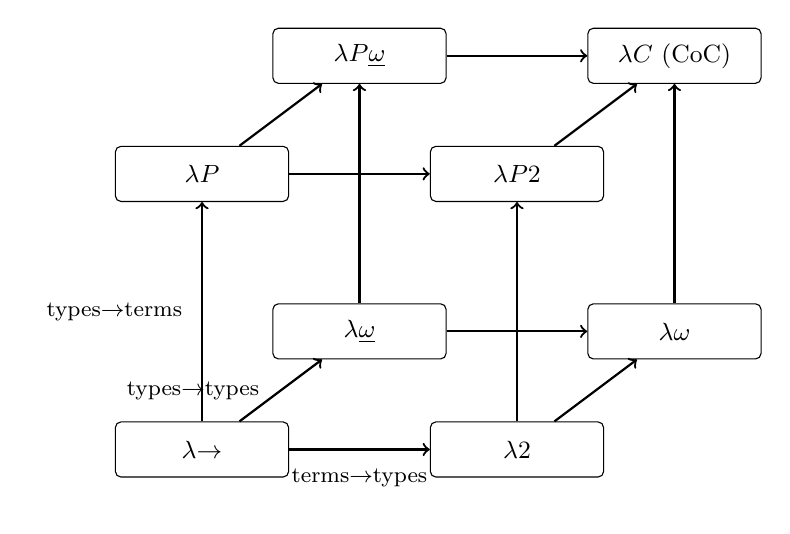
\begin{tikzpicture}[
  every node/.style={draw, rectangle, rounded corners=2pt, minimum width=2.2cm, minimum height=0.7cm, font=\small},
  edge/.style={->, thick},
  scale=1.0
]

% Back face (bottom)
\node (lambda) at (0,0) {$\lambda{\to}$};
\node (lambda2) at (4,0) {$\lambda{2}$};
\node (lambdaU) at (2,1.5) {$\lambda\underline{\omega}$};
\node (lambdaW) at (6,1.5) {$\lambda{\omega}$};

% Front face (top)
\node (lambdaP) at (0,3.5) {$\lambda{P}$};
\node (lambdaP2) at (4,3.5) {$\lambda{P2}$};
\node (lambdaPU) at (2,5) {$\lambda{P\underline{\omega}}$};
\node (CC) at (6,5) {$\lambda{C}$ (CoC)};

% Bottom face edges
\draw[edge] (lambda) -- (lambda2) node[midway,below,draw=none,font=\footnotesize] {terms$\to$types};
\draw[edge] (lambda) -- (lambdaU) node[midway,left,draw=none,font=\footnotesize] {types$\to$types};
\draw[edge] (lambda2) -- (lambdaW);
\draw[edge] (lambdaU) -- (lambdaW);

% Top face edges
\draw[edge] (lambdaP) -- (lambdaP2);
\draw[edge] (lambdaP) -- (lambdaPU);
\draw[edge] (lambdaP2) -- (CC);
\draw[edge] (lambdaPU) -- (CC);

% Vertical edges (types depend on terms)
\draw[edge] (lambda)  -- (lambdaP)  node[midway,left,draw=none,font=\footnotesize] {types$\to$terms};
\draw[edge] (lambda2) -- (lambdaP2);
\draw[edge] (lambdaU) -- (lambdaPU);
\draw[edge] (lambdaW) -- (CC);

\end{tikzpicture}
\end{center}

The corners and their names:
\begin{itemize}
    \item $\lambda{\to}$: The simply typed lambda calculus. Only terms depend on terms.
    \item $\lambda{2}$: System F. Adds terms depending on types (polymorphism).
    \item $\lambda\underline{\omega}$: Adds type constructors (types depending on types), but not polymorphism.
    \item $\lambda\omega$: System F$\omega$. Both polymorphism and type constructors.
    \item $\lambda P$: The LF logical framework. Adds dependent types, but only simple polymorphism.
    \item $\lambda P2$: Adds both dependent types and polymorphism.
    \item $\lambda P\underline{\omega}$: Adds dependent types and type constructors.
    \item $\lambda C$: The \textbf{Calculus of Constructions} (CoC). All four features. The most powerful corner of the cube.
\end{itemize}

The Calculus of Constructions, developed by Thierry Coquand and G\'{e}rard Huet in 1988, is the foundation for the Coq proof assistant (now renamed Rocq). Lean 4's core is also based on a variant. It is the culmination of the lambda cube: terms can depend on terms, types can depend on types, terms can depend on types, and types can depend on terms. Everything can depend on everything.

\begin{keyinsight}[The Cube in Perspective]
The lambda cube is not just a classification; it shows that dependent types are the natural continuation of a line of thinking that starts with simple functions. Each step adds a new kind of dependency. The final step --- types depending on terms --- is the one that unlocks the full power of the system and, as we will see, erases the boundary between programming and proving.
\end{keyinsight}

\section{Types and Programs in the Same World}

In all the type systems we have seen so far, there was a clean separation: types live in one layer, values live in another. You write \code{int x = 5} and the type \code{int} and the value \code{5} inhabit different conceptual worlds.

In dependent type theory, this separation \emph{dissolves}. When a type can mention a value (like \code{Vec(A, n)} mentioning the value $n$), types and values must live in the same syntactic world. The language used to write types and the language used to write programs are the same language.

This has a profound consequence for type checking.

\subsection*{Type Checking Requires Evaluation}

Recall from Chapter 3 that type checking is a static process: you analyse the source code without running it, and determine whether the types are consistent. With simple types, this is easy. With polymorphism, it requires unification, but it is still decidable.

With dependent types, the type checker must compare types like $\text{Vec}(A, m + n)$ and $\text{Vec}(A, n + m)$. Are these the same type? Well, $m + n = n + m$ for natural numbers, so yes. But the type checker must \emph{know} this arithmetic fact. It must evaluate and normalise expressions that appear inside types.

More generally: two types are equal if their \emph{normal forms} are the same. To determine the normal form, the type checker runs a simplification process that is essentially a small interpreter. This is called \textbf{definitional equality} or \textbf{conversion}.

\begin{warning}[Type Checking with Full Dependent Types is Undecidable]
If you allow arbitrary programs to appear inside types, and arbitrary programs can be non-terminating, then type checking can loop forever. The type checker needs to evaluate expressions inside types, and if those expressions diverge, the type checker diverges too.

This is not a theoretical curiosity. It is the reason that most dependently typed languages require programs to be \textbf{total} (every function must terminate on all inputs). In Agda and Coq, you cannot write an infinite loop in the type language --- the system enforces termination using a \textbf{termination checker} (typically based on the \emph{structural recursion} criterion: recursive calls must be on strictly smaller arguments).
\end{warning}

This totality requirement is a significant restriction. It means that, for example, Agda is not Turing-complete in the usual sense: you cannot write programs that loop forever. You can write interpreters for Turing-complete languages \emph{within} Agda, and you can reason about them, but the metalanguage itself must terminate.

From a programmer's perspective, this might feel limiting. But from a mathematical perspective, it makes sense: we want every term in the language to denote a well-defined value. Non-termination is a kind of value (bottom, $\bot$), and including it collapses the careful logical structure that gives dependent types their power.

\section{Dependent Types in Practice: Idris and Agda}

Let us now look at actual code in languages with full dependent types. We will use both Idris 2 (which is designed to be a practical programming language with dependent types, inspired by Haskell) and Agda (which is more proof-oriented but excellent for understanding the theory).

\subsection{Safe \texttt{head} in Idris}

\begin{lstlisting}[style=haskell]
-- Idris 2

-- The standard Vect type, built into Idris
-- data Vect : Nat -> Type -> Type where
--   Nil  : Vect 0 a
--   (::) : a -> Vect n a -> Vect (S n) a

-- Safe head: requires the vector to be non-empty
-- The length is at least 1 (it is S n for some n)
safeHead : Vect (S n) a -> a
safeHead (x :: _) = x
-- No other case needed! Vect 0 a has no elements,
-- so the empty case is impossible.
\end{lstlisting}

Notice there is no case for the empty vector. In ordinary Haskell, omitting a case would be a partial function warning and a potential runtime error. In Idris, it is \emph{correct}: the type \code{Vect (S n) a} is the type of non-empty vectors, and the empty constructor \code{Nil} has type \code{Vect 0 a}, which does not match \code{Vect (S n) a} for any $n$. The compiler knows the case is exhaustive even with only one branch.

\subsection{Safe Indexing in Idris}

\begin{lstlisting}[style=haskell]
-- Idris 2

-- Fin n: the type of natural numbers < n
-- data Fin : Nat -> Type where
--   FZ : Fin (S n)          -- zero is < S n for any n
--   FS : Fin n -> Fin (S n) -- if i < n then i+1 < S n

-- Safe index: the index type guarantees it is in bounds
index : Fin n -> Vect n a -> a
index FZ     (x :: _)  = x
index (FS i) (_ :: xs) = index i xs

-- Example usage:
-- index FZ [1,2,3]          -- returns 1, type: Fin 3 -> Vect 3 Int -> Int
-- index (FS FZ) [1,2,3]     -- returns 2
-- index (FS (FS (FS FZ))) [1,2,3]  -- TYPE ERROR: Fin 4 doesn't fit Fin 3
\end{lstlisting}

The out-of-bounds case is not a runtime error --- it is a \emph{compile-time type error}. You cannot even construct the ill-typed index. \code{FZ} has type \code{Fin (S n)}, so the smallest possible \code{Fin} type is \code{Fin 1}. \code{Fin 0} is empty (no constructor can produce it), making the empty vector case again impossible to call.

\subsection{Matrix Multiplication in Idris}

\begin{lstlisting}[style=haskell]
-- Idris 2

-- A matrix is a vector of rows, each row a vector of columns
Matrix : Nat -> Nat -> Type -> Type
Matrix m n a = Vect m (Vect n a)

-- Transpose: swap rows and columns
-- Input: m x n, Output: n x m
transpose : Matrix m n a -> Matrix n m a
transpose [] = replicate _ []
transpose (row :: rows) = zipWith (::) row (transpose rows)

-- Dot product of two equal-length vectors
dot : Num a => Vect n a -> Vect n a -> a
dot []        []        = 0
dot (x :: xs) (y :: ys) = x * y + dot xs ys

-- Matrix multiply: (m x k) times (k x n) gives (m x n)
-- The inner dimension k MUST match --- enforced by types!
matMul : Num a => Matrix m k a -> Matrix k n a -> Matrix m n a
matMul rows cols =
  let cols' = transpose cols
  in map (\row => map (dot row) cols') rows

-- This would be a TYPE ERROR:
-- matMul (3x4 matrix) (5x2 matrix)  -- inner dims 4 /= 5
\end{lstlisting}

The type signature \code{Matrix m k a -> Matrix k n a -> Matrix m n a} captures the entire mathematical specification of matrix multiplication. The inner dimension $k$ appears in both inputs but not in the output, enforcing that they must match. Pass a $3 \times 4$ matrix and a $5 \times 2$ matrix, and you get a type error --- no runtime exception, no garbage output, just a clean compile-time rejection.

\subsection{A Verified Sorting Function in Agda}

Agda pushes the idea further, letting us write programs together with proofs of their correctness:

\begin{lstlisting}[style=haskell]
-- Agda (pseudocode approximation for readability)

-- A sorted list is either empty, a singleton,
-- or a cons where the head <= the head of the tail
data Sorted : List Nat -> Set where
  sorted-nil  : Sorted []
  sorted-one  : (x : Nat) -> Sorted [ x ]
  sorted-cons : (x y : Nat) -> (xs : List Nat)
             -> x <= y -> Sorted (y :: xs)
             -> Sorted (x :: y :: xs)

-- insert-sort produces a Sorted list
-- The TYPE guarantees correctness!
insertSort : (xs : List Nat) -> Sigma (List Nat) Sorted
insertSort xs = ...  -- implementation
\end{lstlisting}

The return type $\Sigma(\text{ys} : \text{List}(\Nat)).\, \text{Sorted}(\text{ys})$ is a pair: a list \emph{together with a proof that it is sorted}. You cannot return a list without also returning a machine-checked proof of sortedness. The type is the specification, and the program is the implementation and proof simultaneously.

\section{C++ Non-Type Template Parameters: Dependent Types in Disguise}

Here is something that might surprise you: you have already been using dependent types, at least in a limited form. C++ non-type template parameters are a form of dependent typing.

\begin{cppconnection}[Non-Type Template Parameters]
When you write \code{template<int N>} in C++, the type parameter \code{N} is a \emph{value} --- not a type, but an integer. The types that depend on \code{N} are dependent types in the sense of type theory.
\end{cppconnection}

\subsection{\texttt{std::array}: The Canonical Example}

\begin{lstlisting}[style=cpp]
#include <array>
#include <cstddef>

// std::array<T, N>: an array of exactly N elements of type T
// N is a VALUE in the type!
std::array<int, 5> a = {1, 2, 3, 4, 5};
std::array<int, 3> b = {10, 20, 30};

// These are DIFFERENT TYPES:
// std::array<int, 5> and std::array<int, 3> are not compatible.
// You cannot pass one where the other is expected.
// a = b;  // Compile error: different types

// Function that requires exactly 5 elements:
void process_five(const std::array<int, 5>& arr) { /* ... */ }

process_five(a);  // OK
// process_five(b);  // Compile error: wrong type
\end{lstlisting}

\typename{std::array<int, 5>} is a dependent type: the type \typename{std::array<int, N>} depends on the value \code{N}. Two arrays with different sizes have different types. This is the same idea as \code{Vect n Int} in Idris.

\subsection{Writing Dependent-Type-Flavoured Templates}

\begin{lstlisting}[style=cpp]
#include <array>
#include <cstddef>
#include <numeric>

// Dot product of two arrays of the SAME length N
// N appears in both parameter types --- they must match!
template<std::size_t N>
double dot_product(const std::array<double, N>& a,
                   const std::array<double, N>& b) {
    double result = 0.0;
    for (std::size_t i = 0; i < N; ++i)
        result += a[i] * b[i];
    return result;
}

// Matrix as a 2D array: dimensions in the type
template<std::size_t Rows, std::size_t Cols>
using Matrix = std::array<std::array<double, Cols>, Rows>;

// Matrix multiply: (M x K) * (K x N) -> (M x N)
// The shared dimension K must match in both inputs
template<std::size_t M, std::size_t K, std::size_t N>
Matrix<M, N> mat_mul(const Matrix<M, K>& A, const Matrix<K, N>& B) {
    Matrix<M, N> result{};
    for (std::size_t i = 0; i < M; ++i)
        for (std::size_t j = 0; j < N; ++j)
            for (std::size_t k = 0; k < K; ++k)
                result[i][j] += A[i][k] * B[k][j];
    return result;
}

int main() {
    Matrix<2, 3> A = {{{1,2,3},{4,5,6}}};
    Matrix<3, 4> B = {{{1,0,0,0},{0,1,0,0},{0,0,1,0}}};

    auto C = mat_mul(A, B);  // C has type Matrix<2,4>

    // Type error at compile time:
    // mat_mul(A, A);  // Error: Matrix<2,3> != Matrix<3,3>
                       // (K must be 3 in B, but A has K=2)
}
\end{lstlisting}

The mismatch in inner dimensions is caught at compile time! The template instantiation fails if \code{K} does not match. This is not as smooth as Idris --- you get a sprawling template error rather than a clean message --- but the \emph{guarantee} is the same.

\subsection{\texttt{template<auto>} in C++17}

C++17 introduced \code{template<auto N>}, allowing non-type template parameters of deduced type, making the connection to value-indexed types even more natural:

\begin{lstlisting}[style=cpp]
// C++17: template<auto V> -- the value AND its type are deduced
template<auto N>
struct RepeatN {
    // This type encodes the value N
    static constexpr auto value = N;
    // We can do arithmetic on N at compile time
    using doubled = RepeatN<N * 2>;
};

RepeatN<5>  r1;   // Encodes the value 5
RepeatN<5L> r2;   // Encodes the value 5L (long int) -- different type!

// Compile-time string literal as a non-type parameter (C++20)
template<std::size_t N>
struct FixedString {
    char data[N];
    constexpr FixedString(const char (&str)[N]) {
        std::copy(str, str + N, data);
    }
};

template<FixedString S>  // A VALUE in the template parameter!
struct Tag { };

Tag<"hello"> t1;  // The string "hello" is PART OF THE TYPE
Tag<"world"> t2;  // Different type from t1
\end{lstlisting}

In C++20, you can have fixed-size strings as non-type template parameters. \code{Tag<"hello">} and \code{Tag<"world">} are distinct types. The value ``hello'' is encoded in the type. This is about as close to full dependent typing as C++ gets --- and it is surprisingly expressive.

\section{\texttt{constexpr} and Compile-Time Computation}

The other half of C++'s approach to dependent typing is \code{constexpr}: the ability to evaluate ordinary code at compile time, and use the results in types.

\subsection{\texttt{constexpr} Functions}

\begin{lstlisting}[style=cpp]
// A constexpr function can be evaluated at compile time
constexpr int factorial(int n) {
    return (n <= 1) ? 1 : n * factorial(n - 1);
}

// Use the result in a template argument (a type index!)
std::array<int, factorial(5)> arr;  // array of 120 elements
                                     // size computed at compile time

// static_assert: compile-time assertion
static_assert(factorial(5) == 120, "factorial(5) should be 120");
static_assert(sizeof(arr) == 120 * sizeof(int));
\end{lstlisting}

\code{constexpr} functions are evaluated at compile time when their arguments are compile-time constants. The results can be used as non-type template arguments --- effectively, as values that appear in types.

\subsection{\texttt{if constexpr}: Types that Depend on Conditions}

\begin{lstlisting}[style=cpp]
// C++17: if constexpr evaluates the condition at compile time
// and selects which branch to compile (the other is discarded)
template<typename T>
auto to_string_smart(T value) {
    if constexpr (std::is_integral_v<T>) {
        return std::to_string(value);      // For ints
    } else if constexpr (std::is_floating_point_v<T>) {
        return std::to_string(value);      // For floats (same here, but could differ)
    } else {
        return std::string(value);         // For strings/string_views
    }
}

// The key point: the return TYPE can differ in each branch.
// if constexpr lets you write code where TYPE is chosen by VALUE (the condition).
\end{lstlisting}

\subsection{Using \texttt{constexpr} to Derive Dependent-Typed Behaviour}

\begin{lstlisting}[style=cpp]
#include <type_traits>
#include <array>

// A type that is either int or double depending on a bool VALUE
template<bool UseDouble>
using NumberType = std::conditional_t<UseDouble, double, int>;

// The type NumberType<true> is double
// The type NumberType<false> is int
// The TYPE depends on the BOOL VALUE

NumberType<true>  x = 3.14;   // x is a double
NumberType<false> y = 42;     // y is an int

// Compute array size at compile time
constexpr std::size_t compute_buffer_size(int level) {
    return (level == 0) ? 64 : (level == 1) ? 256 : 1024;
}

template<int Level>
struct Cache {
    // The SIZE of this array is determined by the VALUE Level
    std::array<char, compute_buffer_size(Level)> buffer;
};

Cache<0> small_cache;   // buffer has 64 bytes
Cache<1> medium_cache;  // buffer has 256 bytes
Cache<2> large_cache;   // buffer has 1024 bytes
\end{lstlisting}

\begin{cppconnection}[C++ as a Limited Dependently-Typed Language]
C++ with \code{constexpr} and non-type template parameters gives you a limited, somewhat awkward form of dependent typing. The limitations are real: you can only use values of certain ``structural'' types as template parameters (integers, enums, pointers, simple structs in C++20), the syntax is verbose, and error messages are notoriously poor. But the \emph{ideas} are the same as in Idris or Agda. When you write \code{std::array<int, N>}, you are writing a dependent type.
\end{cppconnection}

\section{Universes and the Type of Types}

We have been saying things like ``the type of $n$ is $\Nat$'' and ``the type of $\text{Vec}(A, n)$ is \ldots what?'' We have also said that in dependent type theory, types are values. If types are values, they must have types too. What is the type of a type?

The naive answer is: introduce a special type called \Type, and say that every type has type \Type. So $\Nat : \Type$, $\Bool : \Type$, $\text{Vec}(\Nat, 3) : \Type$, and so on.

But then what is the type of \Type\ itself? If $\Type : \Type$, we have a problem: \textbf{Girard's paradox}, the type-theoretic analogue of Russell's paradox. The system becomes logically inconsistent --- you can derive a proof of False, which means you can prove anything. A type system that proves everything is useless as a logic and unreliable as a type system.

\begin{definition}[Universe Hierarchy]
To avoid Girard's paradox, dependent type theories introduce a \textbf{hierarchy of universes}:
\[
\Type_0 : \Type_1 : \Type_2 : \Type_3 : \cdots
\]
Ordinary types (like $\Nat$, $\Bool$, $\text{Vec}(\Nat, 5)$) live in $\Type_0$. The type $\Type_0$ itself lives in $\Type_1$. The type $\Type_1$ lives in $\Type_2$. And so on, ad infinitum.
\end{definition}

This is the standard solution, due to Martin-L\"{o}f. Each universe is a \emph{type of types}, but at a level below it. There is no universal ``type of all types'' that includes itself, just as in ZF set theory there is no ``set of all sets.''

In practice, most proof assistants implement \textbf{universe polymorphism}: functions and definitions can be parametrised by a universe level, so you do not have to manually track levels most of the time. Agda and Lean both have universe polymorphism. Coq has something similar called the sort system with automatic universe constraint propagation.

\begin{keyinsight}[Universes in Practice]
You encounter universes mainly when you write very generic, highly polymorphic code in Agda, Coq, or Lean. For most programming purposes, you can treat \Type\ as ``the type of ordinary types'' and not worry about the hierarchy. But understanding why the hierarchy exists --- to avoid paradox --- illuminates a deep connection between type theory and the foundations of mathematics.
\end{keyinsight}

\section{Martin-L\"{o}f Type Theory}

The foundational framework that underlies Agda, Coq, Lean, and the entire field of dependent types is \textbf{Martin-L\"{o}f Type Theory} (MLTT), developed by the Swedish logician and mathematician Per Martin-L\"{o}f beginning in the early 1970s.

Martin-L\"{o}f's original motivation was foundational: he wanted a constructive foundation for mathematics that was both logically sound and computationally meaningful. His starting point was the \textbf{Curry-Howard correspondence} (which we explore in depth in Chapter 11): the observation that propositions correspond to types and proofs correspond to programs.

\subsection*{Core Components of MLTT}

\begin{enumerate}
    \item \textbf{Pi types} $\Pi(x : A).\, B(x)$: dependent function types, as described above. Under the Curry-Howard correspondence, these are universal quantifiers: a proof of ``for all $x : A$, $P(x)$'' is a function that takes any $x : A$ and produces a proof of $P(x)$.

    \item \textbf{Sigma types} $\Sigma(x : A).\, B(x)$: dependent pair types. Under Curry-Howard, these are existential quantifiers: a proof of ``there exists $x : A$ such that $P(x)$'' is a pair of an $x$ and a proof that $P(x)$ holds.

    \item \textbf{Identity types} $\text{Id}_A(a, b)$: the type whose inhabitants are \emph{proofs that $a$ and $b$ are equal}. This is the most subtle component. It lets you express and prove equalities as types. A function of type $\text{Id}_\Nat(m + n,\, n + m)$ is a proof that addition is commutative. Modern homotopy type theory (HoTT) takes this idea much further.

    \item \textbf{Inductive families}: the generalisation of ordinary inductive types (like lists and trees) to the dependent setting. Instead of just \code{List A}, you can define families like \code{Vec A n} by induction on the natural number $n$. Inductive families are how you define \code{Fin}, \code{Vec}, \code{Sorted}, and all the other dependently-typed data structures we have discussed.

    \item \textbf{Universes}: the hierarchy $\Type_0 : \Type_1 : \cdots$ to avoid paradox, as described above.
\end{enumerate}

\subsection*{Intensional vs.\ Extensional Type Theory}

One subtlety of MLTT is worth mentioning: the distinction between \textbf{intensional} and \textbf{extensional} versions.

In \emph{extensional} MLTT, two functions are equal if they return equal results on all inputs (the mathematical definition of equality for functions). This is very natural mathematically, but it makes type checking undecidable.

In \emph{intensional} MLTT (used by Agda, Coq, Lean), the identity type $\text{Id}(a, b)$ is \emph{not} automatically inhabited just because $a$ and $b$ are definitionally equal. You must prove equalities that go beyond definitional computation. This makes type checking decidable (given termination), at the cost of requiring more explicit proof work.

\subsection*{Brief History}

\begin{itemize}
    \item \textbf{1972--1984}: Per Martin-L\"{o}f develops several versions of type theory, progressively refining the framework. His 1984 lecture notes (``Intuitionistic Type Theory'') remain a foundational reference.
    \item \textbf{1988}: Coquand and Huet introduce the Calculus of Constructions, the most powerful corner of the lambda cube.
    \item \textbf{1989}: The Coq proof assistant (now Rocq) is begun by Huet and G\'{e}rard Huet's group at INRIA, based on the Calculus of Inductive Constructions (an extension of CoC with inductive types).
    \item \textbf{2007}: Agda 2 is released by Ulf Norell, making dependently-typed programming accessible with a Haskell-like syntax.
    \item \textbf{2013}: The Homotopy Type Theory book is published, a landmark collaborative effort connecting MLTT to algebraic topology.
    \item \textbf{2013}: Idris 1 is released by Edwin Brady, designed specifically as a \emph{programming language} (not just a proof assistant) with full dependent types.
    \item \textbf{2021}: Lean 4 is released, with a mathlib library containing thousands of verified mathematical theorems.
\end{itemize}

MLTT is not just a historical artifact. It is an active research area, influencing programming language design, formalised mathematics, and the foundations of computer science.

\section{The Curry-Howard Correspondence: A Preview}

We will dedicate all of Chapter 11 to this, but we should mention it here because it is inseparable from dependent types.

The Curry-Howard correspondence (also called the propositions-as-types or proofs-as-programs interpretation) says:

\begin{center}
\begin{tabular}{ccc}
\toprule
\textbf{Logic} & & \textbf{Type Theory} \\
\midrule
Proposition $P$ & $\longleftrightarrow$ & Type $P$ \\
Proof of $P$ & $\longleftrightarrow$ & Term of type $P$ \\
$P \wedge Q$ & $\longleftrightarrow$ & $P \times Q$ (product type) \\
$P \vee Q$ & $\longleftrightarrow$ & $P + Q$ (sum type) \\
$P \Rightarrow Q$ & $\longleftrightarrow$ & $P \to Q$ (function type) \\
$\forall x.\, P(x)$ & $\longleftrightarrow$ & $\Pi(x : A).\, P(x)$ \\
$\exists x.\, P(x)$ & $\longleftrightarrow$ & $\Sigma(x : A).\, P(x)$ \\
\bottomrule
\end{tabular}
\end{center}

Dependent types are what make the bottom two rows possible. Pi types are universal quantifiers; Sigma types are existential quantifiers. A dependently-typed programming language is simultaneously a logic: programs are proofs, and types are propositions.

This is why Coq, Agda, and Lean are called \emph{proof assistants} as well as programming languages. You can write programs and prove theorems in the same language, with the type checker serving as both a compiler and a proof verifier.

\section{Why Most Languages Don't Have Full Dependent Types}

If dependent types are so powerful, why does your everyday programming language --- Java, Python, Rust, Go, C++, even Haskell --- not have them?

The reasons are multiple, interconnected, and worth understanding carefully.

\subsection{Type Checking Complexity and Undecidability}

With full dependent types, type checking can require evaluating arbitrary programs, and (as we discussed) arbitrary programs can fail to terminate. To make type checking decidable, you must restrict the language --- typically by requiring all programs to terminate.

Even with termination guarantees, the type checker for a dependently-typed language is dramatically more complex than for a simple or even polymorphic language. It must include:
\begin{itemize}
    \item A normaliser for expressions that appear in types.
    \item A unification algorithm that operates up to definitional equality.
    \item A termination checker to ensure all recursive functions terminate.
    \item Universe level inference and constraint solving.
\end{itemize}

This is a substantial engineering undertaking, and the resulting type checkers are slower and more complex than those for simpler type systems.

\subsection{Totality Requirement}

As mentioned, dependent type systems typically require all programs to be total: every function must terminate on every input. This rules out many ordinary programming patterns:

\begin{itemize}
    \item You cannot write a simple loop that waits for a network packet. (Use monadic IO with explicit effect tracking.)
    \item You cannot write a general fixpoint combinator $Y$. (Recursion must be structural or guarded.)
    \item You cannot have general recursive types without sized types or productivity guarantees.
\end{itemize}

For a proof assistant, totality is a feature: you need termination to ensure that proofs are well-founded. For a general-purpose programming language, it is a significant constraint. Idris threads the needle by allowing \code{partial} annotations (opt-out of totality checking for specific functions), but this is a pragmatic compromise.

\subsection{The Learning Curve and Ergonomics}

Dependent types require thinking about types in a fundamentally new way. The type of a function is not just its input and output types --- it is a precise mathematical specification of its behaviour. Writing code with dependent types means simultaneously writing the program and its specification.

This is powerful but difficult. Writing matrix multiplication in Idris is more work than writing it in Python, because you are also encoding a correctness proof. For many applications, this level of rigour is not necessary and the development cost is too high.

Error messages in dependently-typed systems are notoriously difficult to read. When a type error involves a failed equality between two normalised dependent types, the error message may display large, complex expressions that are difficult to parse without deep system knowledge.

\subsection{The Influence on Every Language}

Despite these challenges, dependent type ideas are spreading into mainstream languages:

\begin{itemize}
    \item \textbf{Rust} has const generics (\code{[T; N]} with \code{N: const usize}), directly analogous to C++'s non-type template parameters.
    \item \textbf{TypeScript} has template literal types and conditional types, allowing some value-level reasoning in types.
    \item \textbf{Python} has \code{Literal} types (\code{Literal[5]} is the type of the value \code{5}), a limited form of dependent typing.
    \item \textbf{Scala} and \textbf{Kotlin} have singleton types and inline functions with reified generics.
    \item \textbf{F\#} has type providers, which generate types from runtime-discovered data schemas.
    \item \textbf{C++} continues to expand its \code{constexpr} and template metaprogramming capabilities with each standard.
\end{itemize}

The full power of dependent types is currently reserved for specialised languages where the benefit (correctness guarantees) outweighs the cost (complexity, totality). But the ideas keep seeping into the mainstream, in simplified forms, as language designers recognise the value of more precise types.

\begin{keyinsight}[Dependent Types: The Frontier of Type Theory]
Dependent types represent the current frontier of practical type theory. They are powerful enough to express any mathematical proposition as a type and any proof as a program. The most safety-critical software --- verified compilers (CompCert), verified operating system kernels (seL4), formalised mathematics (Lean's Mathlib) --- uses these ideas. Understanding them gives you a window into both the future of programming languages and the deepest connections between computation and logic.
\end{keyinsight}

\section{Connecting the Thread: From Chapter 1 to Here}

Let us take a moment to see how far we have come.

In Chapter 1, we defined a type as a set of values with operations. Types were labels: \code{int} labels integers, \code{bool} labels booleans. Simple.

Then we added functions: types can describe arrows between sets of values. Then products and sums: types can describe structured and alternative data. Then polymorphism: types can have \emph{type} parameters, letting a single function work for many types. Then type classes and constraints: types can carry requirements and capabilities.

And now: types can depend on \emph{values}. The length of a vector is not just a runtime number --- it is part of the vector's type. A natural number less than $n$ has a type that encodes the bound. A sorted list carries a machine-checked proof of sortedness in its type.

Each chapter has been expanding the expressive power of the type language. Dependent types are the culmination: a type language that is as powerful as the programming language itself, because they \emph{are} the same language.

\begin{figure}[h!]
\centering
\begin{tikzpicture}[
  node distance=0.9cm,
  box/.style={draw, rounded corners, fill=blue!8, minimum width=5cm, minimum height=0.7cm, font=\small, align=center}
]
\node[box] (st) {Simple Types ($A$, $A \to B$, $A \times B$, $A + B$)};
\node[box, below=of st] (pt) {Parametric Polymorphism ($\forall \alpha.\, T$)};
\node[box, below=of pt] (tc) {Type Classes / Constraints ($C \Rightarrow T$)};
\node[box, below=of tc] (hk) {Higher-Kinded Types (Type Constructors)};
\node[box, below=of hk, fill=blue!20, font=\small\bfseries] (dt) {Dependent Types ($\Pi$, $\Sigma$, Indexed Families)};

\foreach \from/\to in {st/pt, pt/tc, tc/hk, hk/dt}
  \draw[->, thick] (\from) -- (\to);

\node[right=0.3cm of st, draw=none, font=\footnotesize, text=gray] {Chapters 1--4};
\node[right=0.3cm of pt, draw=none, font=\footnotesize, text=gray] {Chapters 5--7};
\node[right=0.3cm of tc, draw=none, font=\footnotesize, text=gray] {Chapter 8};
\node[right=0.3cm of hk, draw=none, font=\footnotesize, text=gray] {Chapter 9};
\node[right=0.3cm of dt, draw=none, font=\footnotesize, text=gray] {Chapter 10};
\end{tikzpicture}
\caption{The progressive enrichment of type languages throughout this book.}
\end{figure}

\section{Exercises}

\begin{exercise}
Consider the type $\text{Vec}(A, n)$ in Idris. Without running any code, determine:
\begin{enumerate}[label=(\alph*)]
    \item What type does \code{Nil} have?
    \item What type does \code{x :: Nil} have, where \code{x : Int}?
    \item What type does \code{append (x :: Nil) (y :: z :: Nil)} have?
    \item Is the expression \code{head Nil} well-typed? Why or why not?
\end{enumerate}
\end{exercise}

\begin{exercise}
In C++, write a function template \code{safe\_get} that takes an \code{std::array<T, N>} and a \code{std::size\_t} index. Use \code{static\_assert} to enforce that the index is a compile-time constant less than \code{N}. (Hint: make the index a template parameter.)

Then discuss: why is this less ergonomic than the Idris \code{index} function with \code{Fin n}? What does Idris provide that C++ templates do not?
\end{exercise}

\begin{exercise}
The Sigma type $\Sigma(n : \Nat).\, \text{Vec}(A, n)$ is said to correspond to a dynamically-sized vector. Compare this to \code{std::vector<A>} in C++. What is the correspondence? What does \code{std::vector} provide that the Sigma type does not? What does the Sigma type guarantee that \code{std::vector} does not?
\end{exercise}

\begin{exercise}
Place each of the following type systems in the lambda cube. Justify your placement:
\begin{enumerate}[label=(\alph*)]
    \item The simply typed lambda calculus.
    \item Haskell (without type families or GADTs).
    \item Haskell with type families and \code{DataKinds}.
    \item C++ templates (non-type parameters included).
    \item Agda.
    \item Java generics.
\end{enumerate}
\end{exercise}

\begin{exercise}
Consider the type $\Sigma(f : \Nat \to \Nat).\, \Pi(n : \Nat).\, f(n) \geq n$. Describe in plain English what a value of this type is. What program would you need to write to produce a value of this type?
\end{exercise}

\begin{exercise}[Programming Challenge]
In Idris 2 (or pseudocode), write the following functions with their most precise dependent types:
\begin{enumerate}[label=(\alph*)]
    \item \code{zip : Vect n a -> Vect n b -> Vect n (a, b)} --- zip two equal-length vectors into a vector of pairs.
    \item \code{take : (k : Nat) -> Vect (k + m) a -> Vect k a} --- take the first $k$ elements.
    \item \code{splitAt : (k : Nat) -> Vect (k + m) a -> (Vect k a, Vect m a)} --- split a vector at position $k$.
\end{enumerate}
For each, explain how the types prevent incorrect implementations.
\end{exercise}

\begin{exercise}
Universe levels: explain in your own words why $\Type : \Type$ leads to paradox (look up ``Girard's paradox'' or ``Russell's paradox'' for inspiration). Then explain how the universe hierarchy $\Type_0 : \Type_1 : \Type_2 : \ldots$ resolves the problem. At what universe level does $\Type_0 \to \Type_0$ (the type of type operators) live?
\end{exercise}

\begin{exercise}[Research]
Look up the CompCert verified C compiler or the seL4 verified microkernel. Both were verified using proof assistants based on dependent type theory. Write a short paragraph describing: what was verified, which proof assistant was used, and what guarantees the verification provides that ordinary testing does not.
\end{exercise}

\begin{takeaway}[Chapter 10 Takeaways]
\begin{itemize}
    \item \textbf{Dependent types} let types depend on values, not just other types. The type $\text{Vec}(A, n)$ encodes the exact length $n$ of a vector in the type itself.

    \item \textbf{Pi types} $\Pi(x : A).\, B(x)$ are dependent function types: the return type varies with the input value. They generalise both ordinary function types ($A \to B$) and polymorphism ($\forall \alpha.\, T$).

    \item \textbf{Sigma types} $\Sigma(x : A).\, B(x)$ are dependent pair types: the type of the second component depends on the value of the first. They generalise ordinary product types and existential types.

    \item The \textbf{lambda cube} organises type systems by what can depend on what. The most powerful corner is the Calculus of Constructions, where terms and types can each depend on both terms and types.

    \item With dependent types, \textbf{type checking requires program evaluation}. To keep type checking decidable, most dependently-typed systems require all programs to be \textbf{total} (terminating on all inputs).

    \item \textbf{C++ non-type template parameters} (\code{template<int N>}, \code{std::array<T,N>}) are a limited but real form of dependent typing, where a type depends on an integer value.

    \item \textbf{Martin-L\"{o}f Type Theory} is the foundational framework, developed in the 1970s. It is the basis for Agda, Coq/Rocq, and Lean.

    \item The \textbf{Curry-Howard correspondence} connects dependent types to logic: Pi types are universal quantifiers, Sigma types are existential quantifiers, and programs are proofs. (More in Chapter 11.)

    \item Dependent types are the \textbf{frontier} of practical type systems. They are used in verified compilers, verified operating systems, and formalised mathematics. Their influence is spreading into mainstream languages in simplified forms.
\end{itemize}
\end{takeaway}
